\documentclass[]{article}

\usepackage{epigraph}
\usepackage{setspace}
\usepackage{changepage}
\usepackage{amssymb}
\usepackage{amsmath}
\usepackage{graphicx}
%\usepackage{hyperref}
\usepackage[backend=bibtex]{biblatex}
\addbibresource{refs.bib}
%opening
\title{Darts}
\author{Max Caragozian}

\begin{document}

\maketitle


\epigraph{The tap-room fire is alight again and a new stock of darts laid in; serviceable and well-feathered, that fly true and will see us into another spring.}{``A Chiltern Autumn'' \cite{1929spectator}}

\section{Introcudction}
When I moved to Rochester this past January, I bought a dartboard and hung it in the basement of my college house. It ended up being a worthwhile purchase, both as a way to get to know my new roommates and as time killer for what ended up being a long, snowy winter. I started reading into the mathematics of darts and came across the paper ``A Statistician Plays Darts''\cite{stat},  which quantifies how a dart thrower's skill affects where he/she should aim. 

In the simplest model, the authors assume that a person throws with a symmetrical bivariate normal distribution. They estimate the function $\mu^*(\sigma)$ that takes in a standard deviation $\sigma$ and outputs a point $\mu$ that maximizes the expected score of a dart thrown with distribution $\mathcal{N}(\mu, \sigma^2)$.

Bad sentence -> Unsurprisingly, the authors found that a person with a very small standard deviation should aim for the triple 20 (T20), as it has the highest point value on the board. The optimal aiming location stays in the T20 until approximately $\sigma=16.9$mm, where the optimal location jumps to the T19, before eventually moving towards the center of the board.

At the outset of this project, my aim was to replicate some of the results of ``A Statistician Plays Darts.''\cite{stat} Along the way, I found that there is more than one way to get there and learned much about global optimization algorithms. This paper documents the several methods I tried, how I implemented them, and how each method 111

\begin{figure}
	\centering
	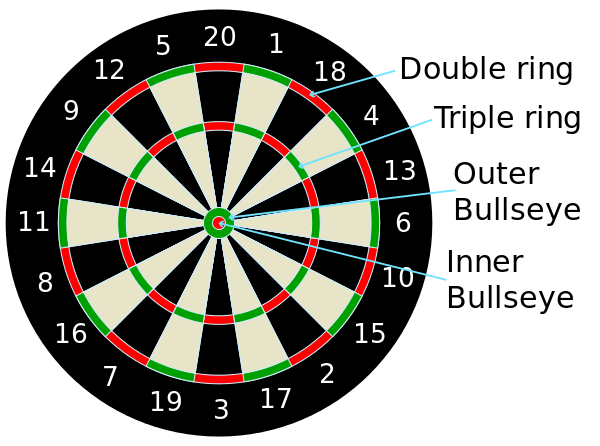
\includegraphics[width=\textwidth]{../images/dartboard_diagram.png}
	\caption{Standard dartboard with point values \cite{diag}}
	\label{fig:diag}
\end{figure}

\section{Brute Force}
Before trying to find $\mu^*(\sigma)$, I wrote code that would find the expected score for someone throwing a dart with a given random distribution. We define a \textit{sector} as a continguous area of the dartboard with a single point value. Examples are the triple 20, the double bullseye, or the portion of single 19 that lies between the outer bullseye ring and the inner triple ring. We define $S$ as the set of all sectors and $X$ as a distribution with PDF $f_x$. To find the expected score of a distribution we compute:


 

\begin{equation}
	E[score(X)] = \sum_{s \in S} \iint_{s} score_s \cdot  f_x(x, y)  dxdy.
	\label{eq:int}
\end{equation}



I used SciPy's \textit{nquad} function to perform the integration. Originally, I used the \textit{dblquad} method, which is specific to double integral, but I ran into a rounding issues when $f_x$ was very small. The \textit{nquad} function allows finer control and fixed the issue. 

With the code implementation of Equation \ref{eq:int}, I could fix $\sigma$ and calculate the expected score of normal distributions centered at many different points across the dartboard. I could then plot the results as a heat map.

\begin{figure}[h]
	\centering
	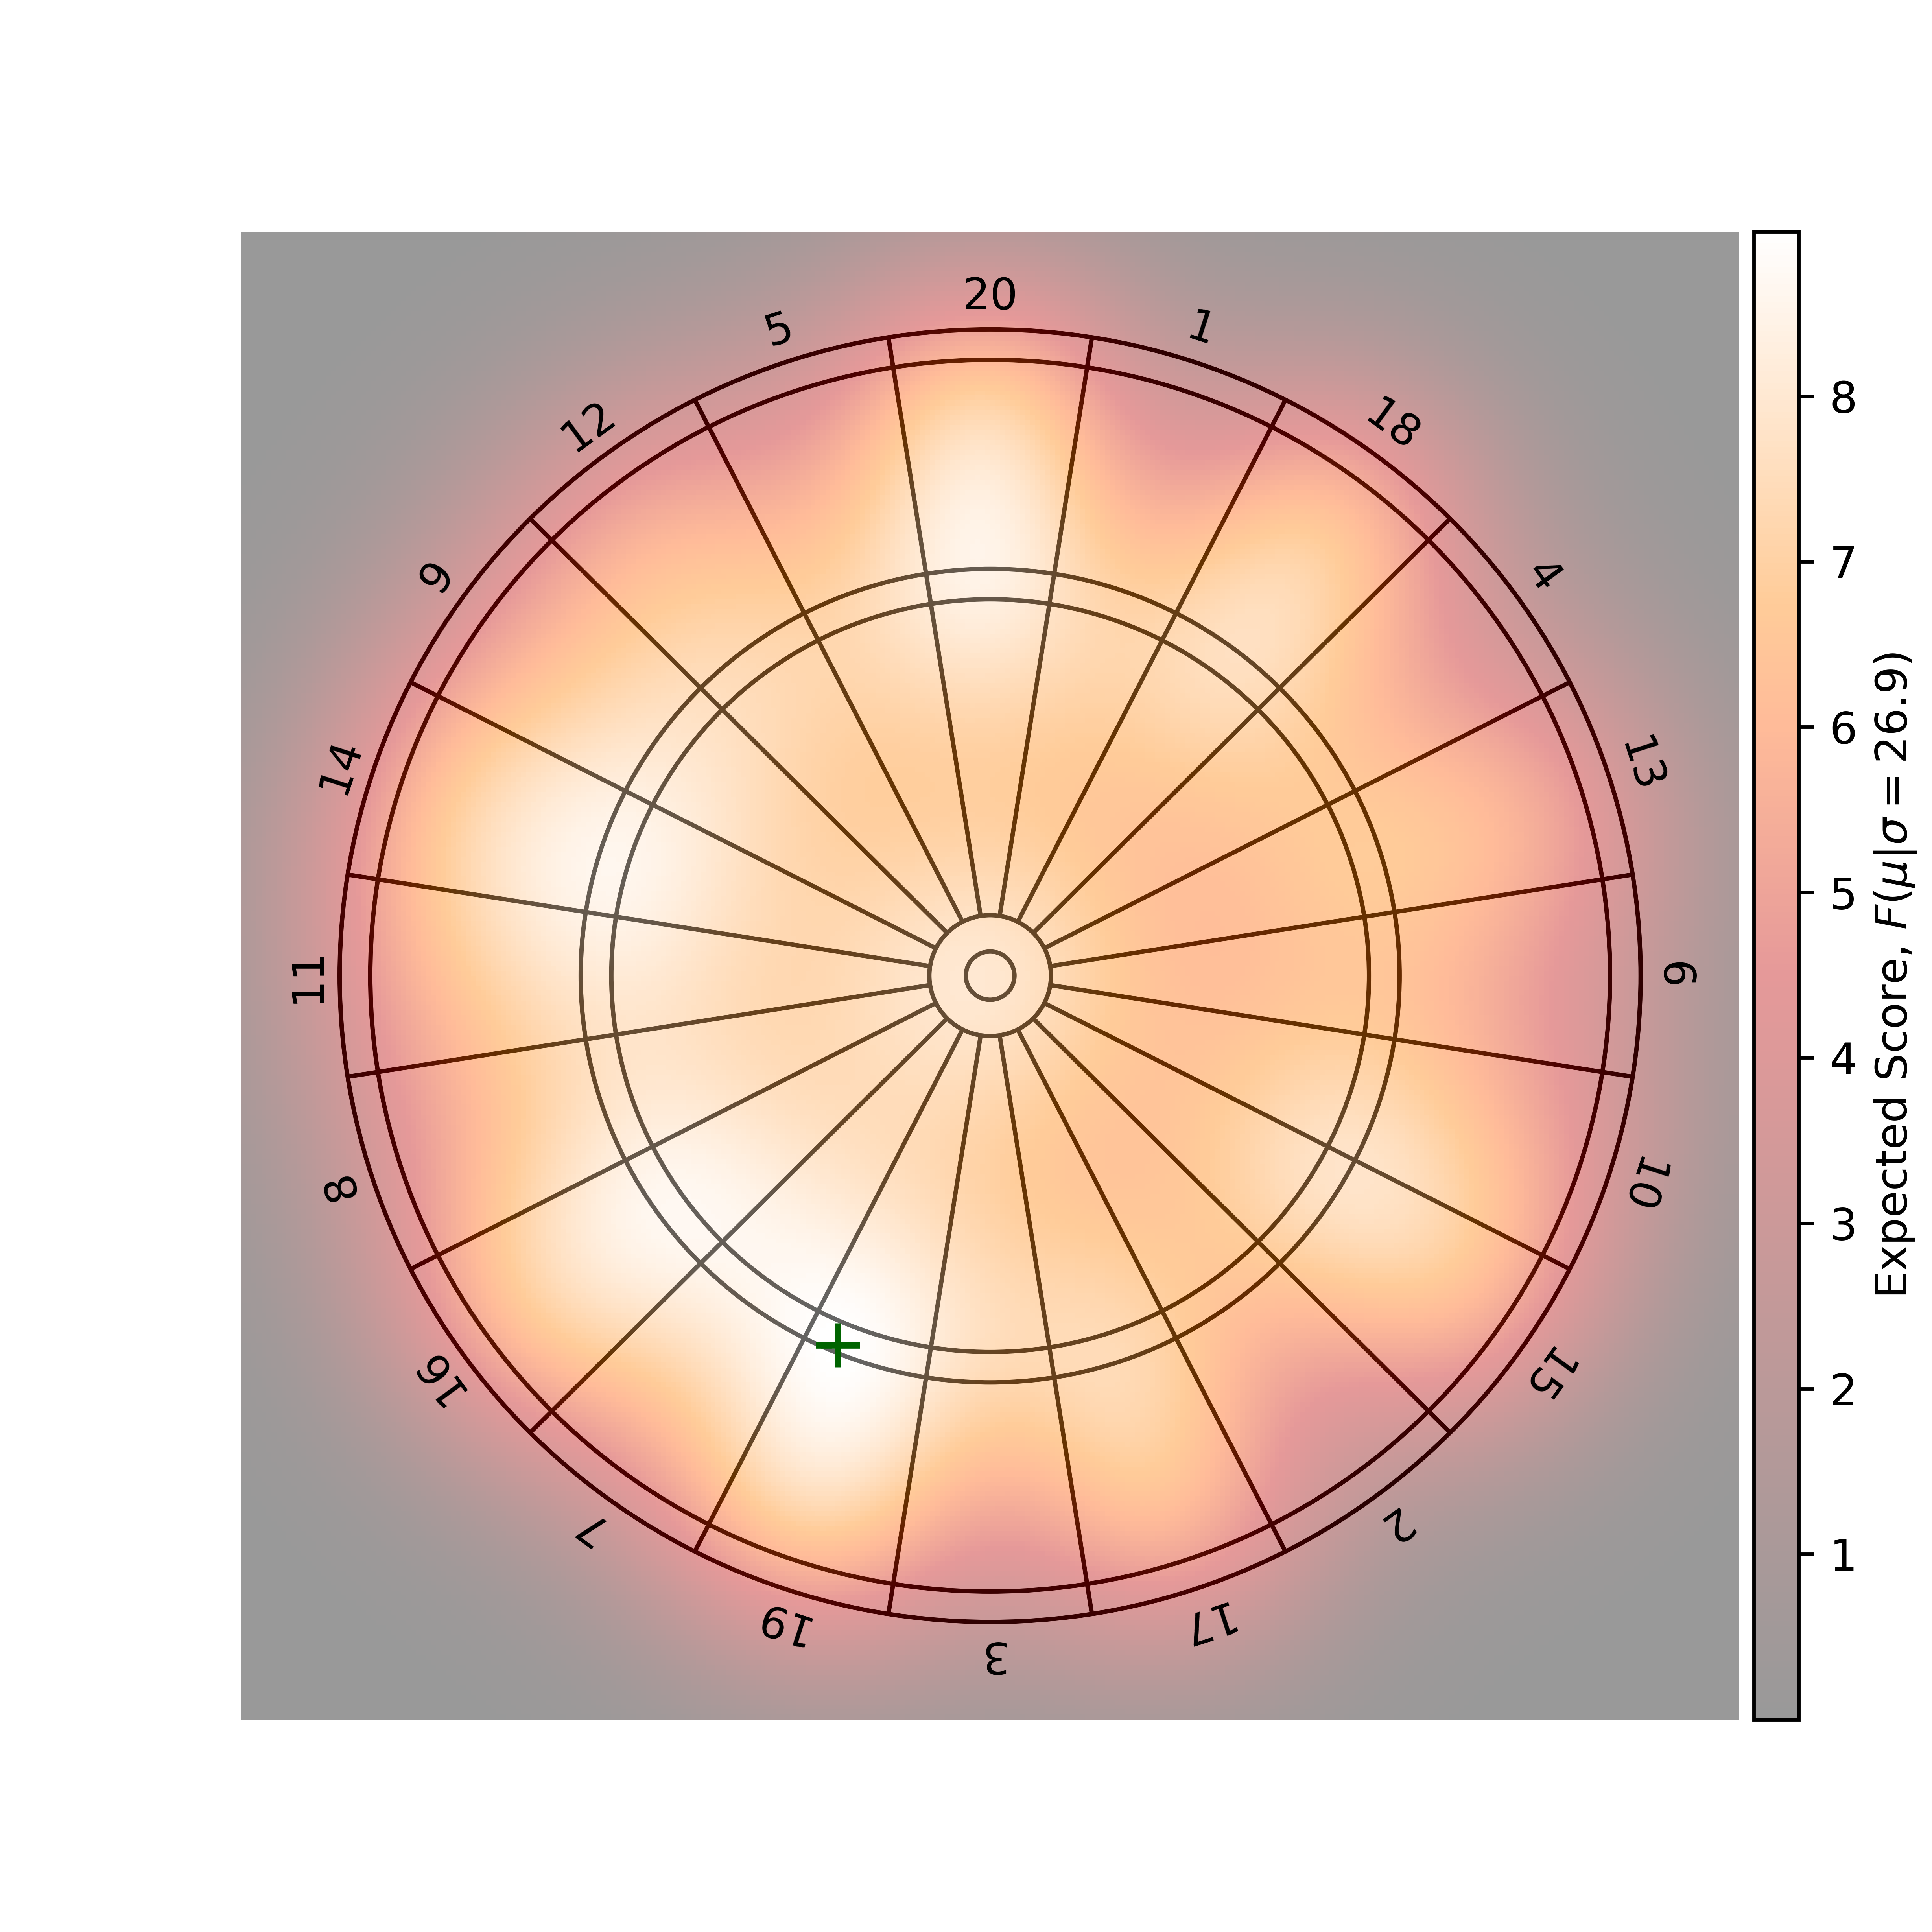
\includegraphics[width=\textwidth]{../images/gist_hear.png}
	\caption{Heatmap for $\sigma = 26.9$. The green \textbf{+} is the location of  $\mathbf{\mu^*}$}
\end{figure}






	

\printbibliography
\end{document}
